% !TEX root = ../../thesis.tex

\cleartoleftpage
\includepdf{../media/chapter_illustration/poppy_prairie_2.pdf}

\chapter{Open diffusion of Poppy} % (fold)
\label{cha:diffusion}

\section{Introduction} % (fold)

Poppy was initially designed with a scientific objective, aiming to be a new experimental platform opening the possibility to systematically study the role of morphology in sensorimotor control, in human-robot interaction and in cognitive development. Yet, until recently it was complicated because building a robot relied on heavy and costly manufacturing techniques. 3D printing has changed the landscape of what is possible: the design of Poppy transposed it to humanoid robotics and we developed complementary open source electronic and software. As we saw in chapter~\ref{cha:changing_morphology}, it allows to explore new body shapes in just a few days.
In addition, it enables and simplifies the experimentation, the reproduction and the modification of the morphology in research laboratories. It also allows collaborative working, sharing and replication of the results between laboratories.

On the scientific aspect, the ambition is to become a reference platform for benchmarking and dissemination of scientific results. Also the simple design of Poppy also targets non-engineering scientists so humanities, biologist and so on can contribute to the robotics field by using Poppy as experimental tool.
Moreover, thanks to the fact that it integrates advanced and yet easily accessible techniques in an embodiment that motivates students and the wider public, this platform also meets a growing societal need: education and training in technologies combining computer science, electronics and mechanics, as well as a training tool to the emergent revolutionary 3D printing process. With its openness, its design and its rather low-cost, Poppy provides a unique context for experimentation and learning of these technologies in a Do-It-Yourself (DIY) approach.
Finally, the possibility to easily modify both the hardware and the software also makes Poppy a useful tool for artistic projects working with interactive computerized installations.

% Poppy is an open source/open science project, even if the technology developed have high potential to be relevant in Art, Education and of course Science, the user community is a paramount of importance. Because the robot and tools own to the community, it is crucial to have a place to exchange idea and works.

The major challenge is now to succeed in the diffusion of the platform in all these fields. As we can see we the Arduino example, the user community is a paramount of importance and both the diffusion strategy and community management tools are critical.

We think this challenge relies on 3 main aspect: create a playful and motivating multidisciplinary community, improve the hardware modularity and integrate Poppy in the maker revolution by using Fablab for production and distribution.


\section{Creating a multidisciplinary community} % (fold)
\label{sec:creating_a_multi}
Toward the creation of such a community, some people are really interesting and have been a great source of inspiration for our work. Among them we can cite Massimo Banzi one of the co-founder of Arduino which spent near 10 years working on the Arduino community. We can also cite Jeff Atwood, co-founder of stack-exchange, he is a software developer who become specialist in creating tool for web community. Along his work he developed a really sight and pragmatic vision of the management of people into a community. The feedback he shares on its blog (ref) is really worth reading for anyone wanting to create a community.

The creation of a Poppy's community began when we released Poppy under open source license (October 2013).
The first interaction people has with the project is the website. We managed to create a nice and simple website on \url{www.poppy-project.org} so experts can see potential of the platform while newbies are not afraid by too much technical information.
Yet this website and the open source release draw a lot of attention and we eventually got submerged by emails and community management. We globally failed to absorb all this enthusiasm as we were not prepared with adapted community tools such as wiki, forum and so on.

\begin{figure}[tb]
\centering
    \subfloat[][Old BBpress forum]{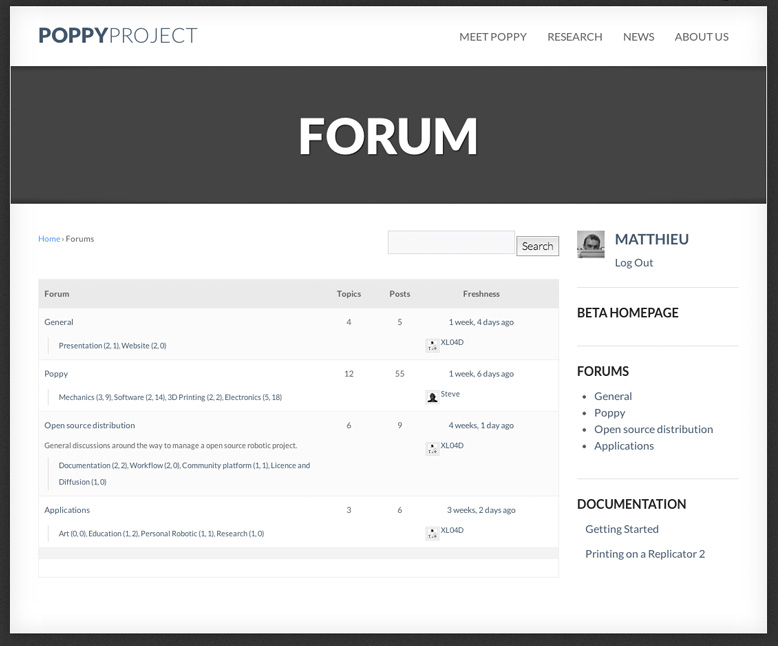
\includegraphics[height=5.2cm]{poppy_forum_bbpress.jpg}}
    \hfil
    \subfloat[][Current Discourse forum]{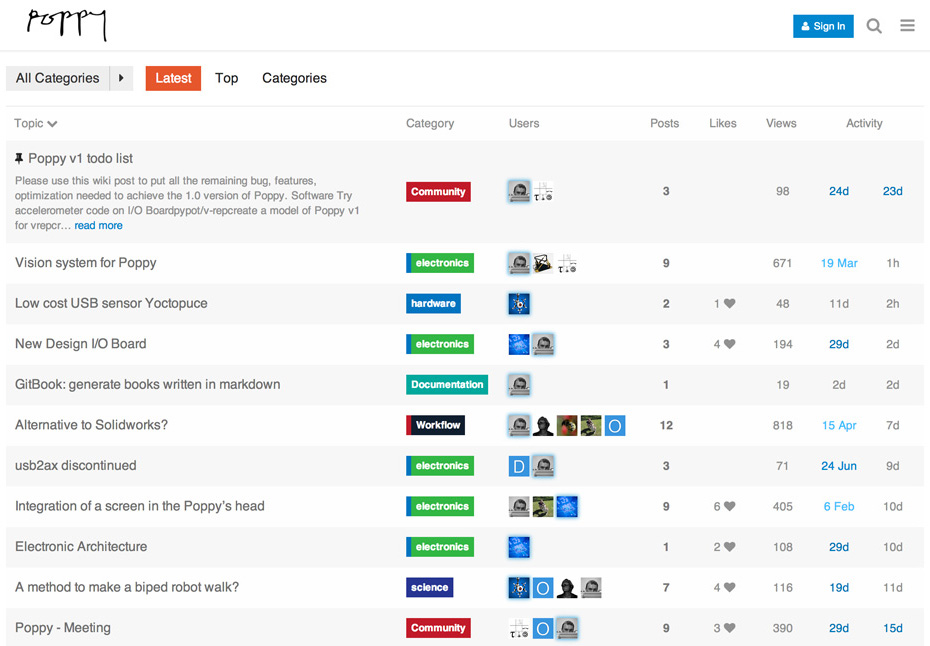
\includegraphics[height=5.2cm]{poppy_forum_discourse.jpg}}
    \caption{Evolution of the forum for the Poppy project}
    \label{fig:poppy_forum}
\end{figure}

Since several months, we set-up a novel forum technology called Discourse\footnote{\url{www.discourse.com}} and created by Jeff Atwood. This forum available on \url{forum.poppy-project.org} greatly help us to manage the community, as it is playful and simple (see \figurename~\ref{fig:poppy_forum}). It is so efficient that we began to use it also for our internal discussions about Poppy's development. These discussions are made public so we can merge time between communication and development.

While this technology solves one of our problems, there are still several others. Firstly, we did not find a wiki technology as simple and playful as Discourse, therefore currently the project lack of documentation (excepted for pypot those documentation is complete).

Secondly, as science project, we naturally decided to use the English as main language for all communication associated with the project. This implies the main website for presenting the project, as well as support on the forum and the current documentation. However, as we can see in the \figurename~\ref{fig:poppy_community}, english-native people only represent the third of the Poppy's community. While English is usually not a problem for Germanic country, we have been confronted to a lack of contribution from Latin countries on our forum. It is especially the case with French educational and artistic communities those never contributed to the forum even after the successful experiments we have had (see chapter~\ref{cha:education} and chapter~\ref{cha:art}).

Following the Arduino example, we now turned our forum multilingual\footnote(see this topic \url{}) by allowing and creating the associated categories for French, German, Italian, Espagnol and Portuguese. We are also currently translating the main website. This work did not yet produce result, but we missed the opportunity during the experiments we had, and we certainly have to wait until the new experiments with education and artist to see the results.

\begin{figure}[tb]
\centering
    \subfloat[][]{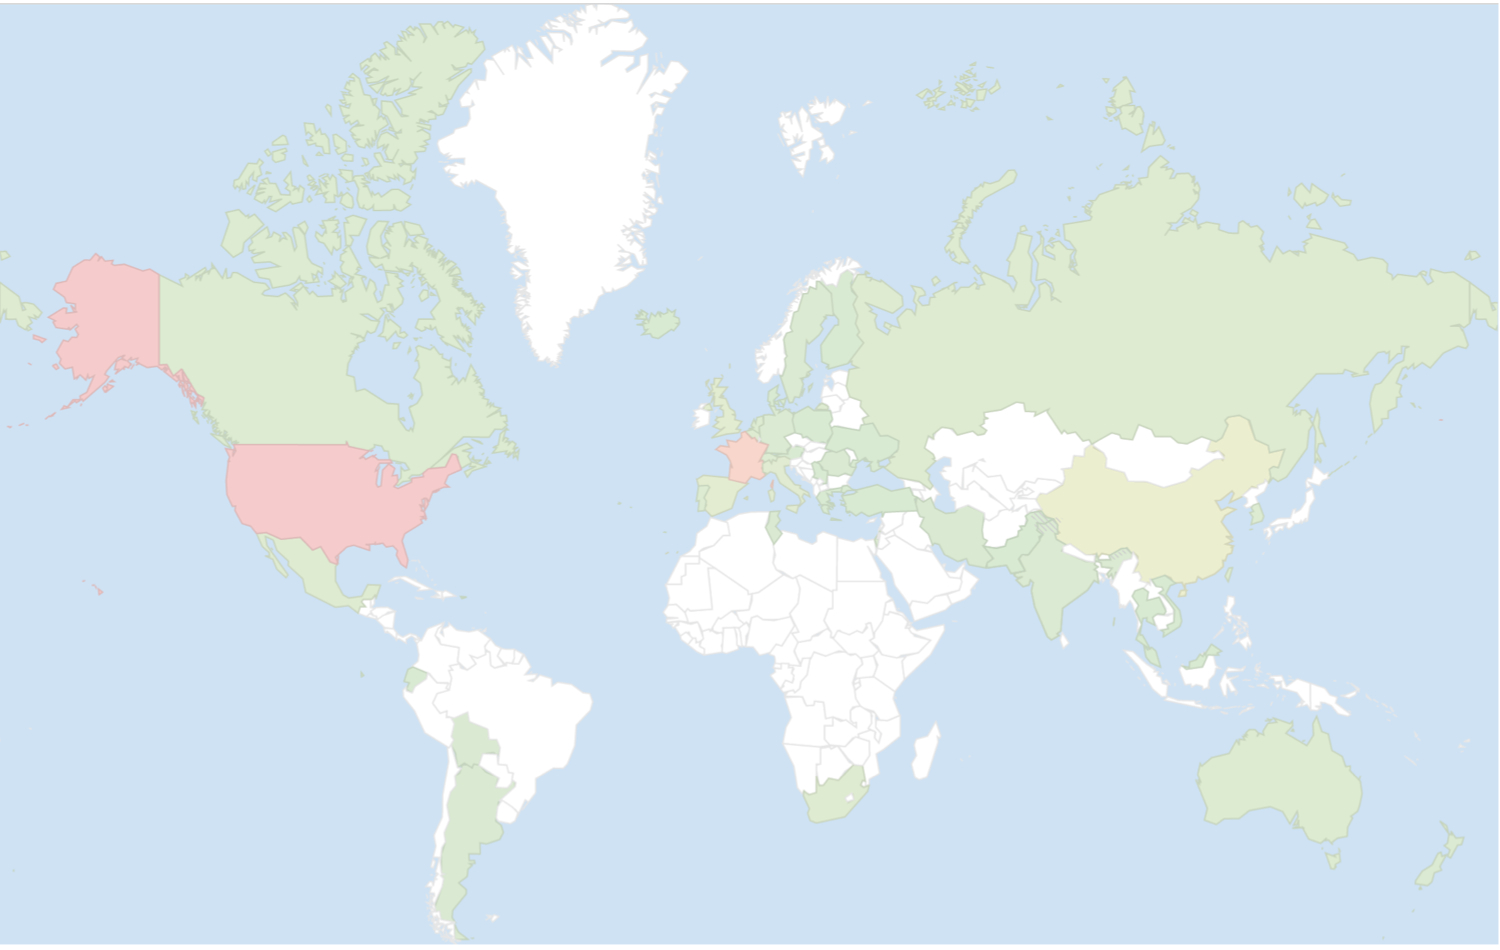
\includegraphics[height=4.5cm]{world_map.jpg}}
    \hfil
    \subfloat[][]{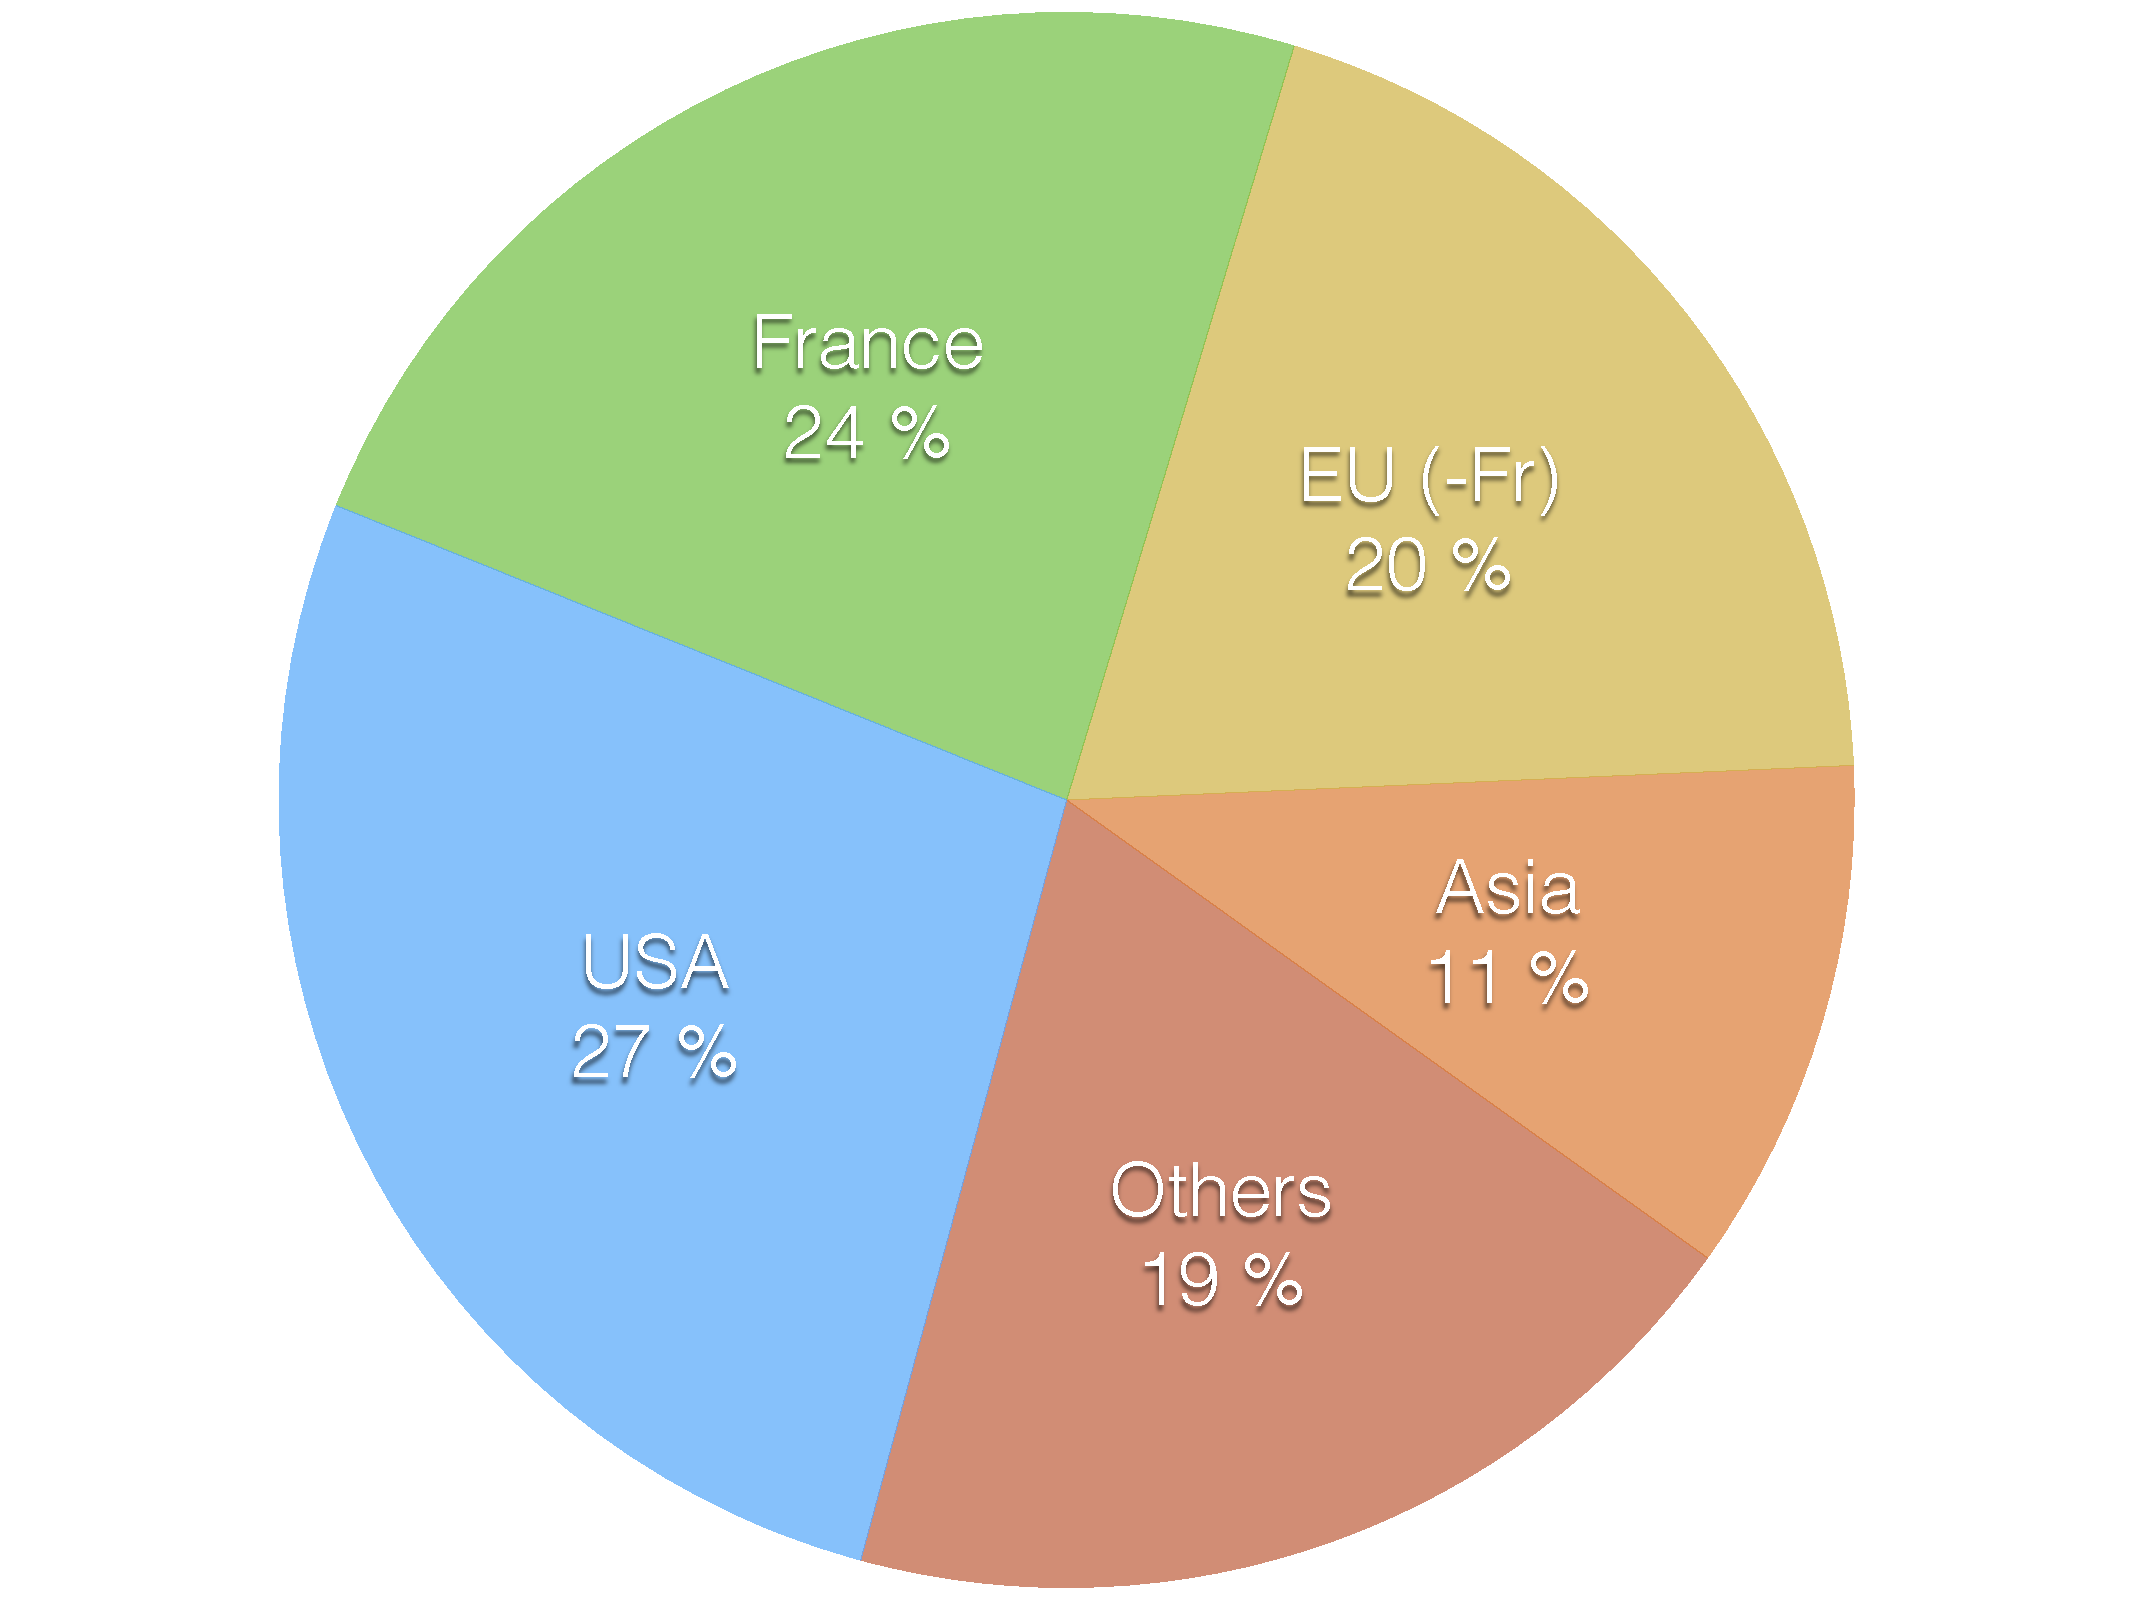
\includegraphics[height=4.5cm]{user_country.pdf}}
    \caption{Activity tracked during October 2013 to February 2014}
    \label{fig:poppy_community}
\end{figure}






% \section{Improve accessibility} % (fold)

% For artists and students

% Heidi referenced the Paradox of the Active User (pdf), which has been around as a concept since 1987. I highly recommend reading the original paper, but if you don't have time, Jakob Nielsen summarizes:

% \begin{formal}
% Users never read manuals but start using the software immediately. They are motivated to get started and to get their immediate task done: they don't care about the system as such and don't want to spend time up front on getting established, set up, or going through learning packages.
% The "paradox of the active user" is a paradox because users would save time in the long term by learning more about the system. But that's not how people behave in the real world, so we cannot allow engineers to build products for an idealized rational user when real humans are irrational. We must design for the way users actually behave.
% \end{formal}

% The assembly of Poppy has several point what indicates to the user how they should mount a part.


\section{Improving the hardware modularity} % (fold)
\label{sec:improve-hardware-modularity}

As we discussed in details in this thesis, Poppy has a modular morphology. This modularity is expressed with all technologies involved. For the mechanics, we use 3D printing techniques allowing to produce quick and low-cost parts. For the electronics, we designed an electronics board based on Arduino allowing to easily plug new sensors. Finally for the software, we built a library using an modular architecture both for the low-level thanks to I/O controllers and for the high-level with primitives paradigms.

As we saw in the chapter REF, this modularity allows for quick experimentation over morphological variants. This functional modularity seems to be enough to allow a wide range of scientific experiments with Poppy and hopefully have real a scientific impact. However, to have an actual impact in the open source community, the technological modularity is essential.

In the software, modularity refers to the manner in which a design is decomposed into different "modules". It is based on the notion of interdependence within modules and independence between modules~\parencite{baldwin2000design}. This concept involves two related ideas: the need to allow work on a given module to be carried out without affecting other modules in the design, a concept known as "loose-coupling", and the need for well-designed "interfaces" between these modules~\parencite{maccormack2006exploring}.

The concept of modularity appears as a fundamental property in the the open source software collaboration. Indeed, code modularity allows the overall project to be divided into much smaller and well-defined tasks that individuals can tackle independently from other tasks and without affecting other aspects of the program~\parencite{narduzzo2008modularity}.

Thus Linus Torvalds, emphasized modularity as a design criterion early in the development of Linux~\parencite{dibona1999open}. Indeed without modularity, it would be improbable that contributors could understand the whole design architecture to have a relevant contribution. It would be difficult to add new features or fix bug without affecting other part of the design. Linux needed to be modular to attract and facilitate a developer community. Code modularity allows partitioning of work among a global pool of developers and facilitates the recruitment of new contributors, as it reduces their learning curve to a subset of modules rather than the entire project~\parencite{fitzgerald2004critical}.

Various efforts by corporations selling proprietary software products to develop additional products through an open source approach have been undertaken.One of the most visible of these efforts was Netscape's 1998 decision to make 'Mozilla', a portion of its browser source code, freely available.This effort encountered severe difficulties in its first year, only receiving approximately two dozen postings by outside developers. Much of the problems appeared to stem from the insufficiently modular nature of the software: reflecting its origins as a proprietary commercial product,the different portions of the program were highly interdependent and interwoven.

For twenty years, the open source software development managed to find efficient workflow. There are now tools, rules and guidelines allowing people to develop together new software fluently.

The hardware modularity is not as developed as the software one because it is not possible to abstract the interface. Hardware components have a global shape, connector type and position, and so on, which make difficult to design efficient interface.

\begin{figure}[tb]
\centering
    \subfloat[][Arduino form factor]{\includegraphics[height=3.5cm]{arduino-shield.png}}
    \hfil
     \subfloat[][Google Ara project]{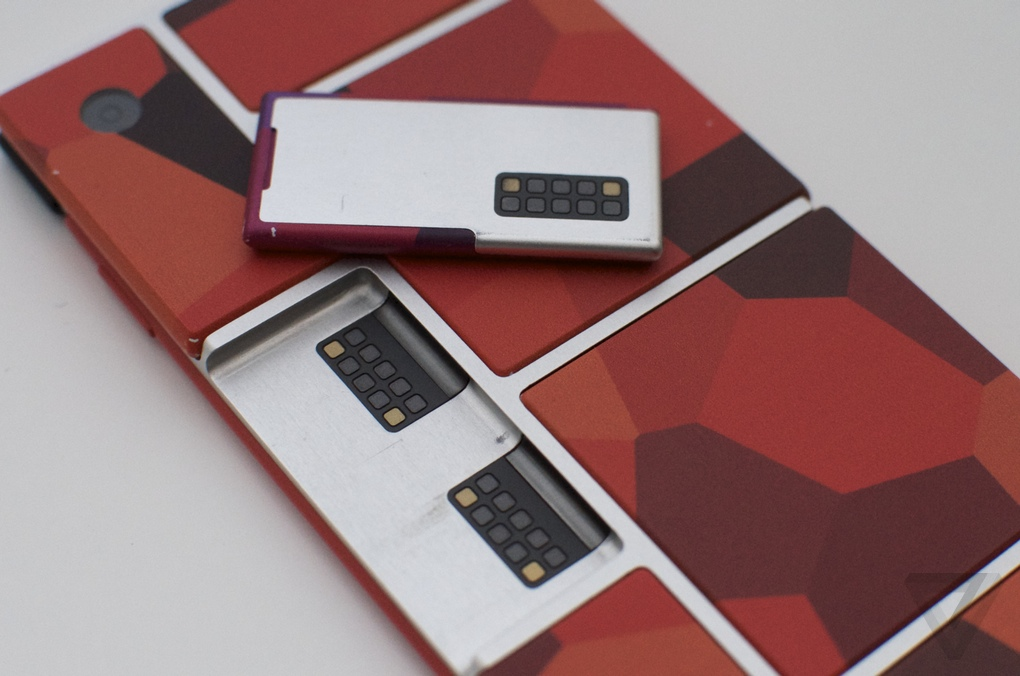
\includegraphics[height=3.5cm]{project-ara.jpg}}\\
    \caption{}
    \label{fig:hardware-modularity}
\end{figure}

Yet some projects have already addressed these challenges. For example, the Arduino boards (Uno, Leonardo, Yun, Mega, Due) share a same footprint (i.e. where are placed the main I/O pins), in this way any shield developed for one of these Arduino board can also be used on other one. This modularity is a lever arm for the community as potential contributors know that the shield they develop and possibly sell will be compatible we several boards and future ones.
Another example is the Google ARA project, it is a smart-phone with modular elements. It is possible to change only the processor or the camera without having to change the whole phone. To achieve such design, they created interface block (see REF). Therefore any modules following the interface rules can be plugged on the phone.

% Add the fact what people should be able to change easily a part of the robot

To improve the potential impact of Poppy for technology we need to follow such ideas. Indeed the methodology to build Poppy allows for modularity but the actual hardware design is interdependent. The functioning of each mechanical part depends also on element connected to it, for example, the way the pelvis is designed changes the mobility of the legs. Also the particular shape of the IO board and the way connectors are placed, are designed to fit in the current design of Poppy's head.

It does not avoid the reuse of such components into other projects but it reduces their relevance. Among all it raise difficulties for potential contributor as they have to understand the whole mechatronics architecture rather than focusing on one precise element.


Thus the new technology development will be more oriented toward hardware modularity. This work is already under process for the two main aspect of the robot.

\begin{figure}[tb]
\centering
    \subfloat[][IO Module schematics (under production)]{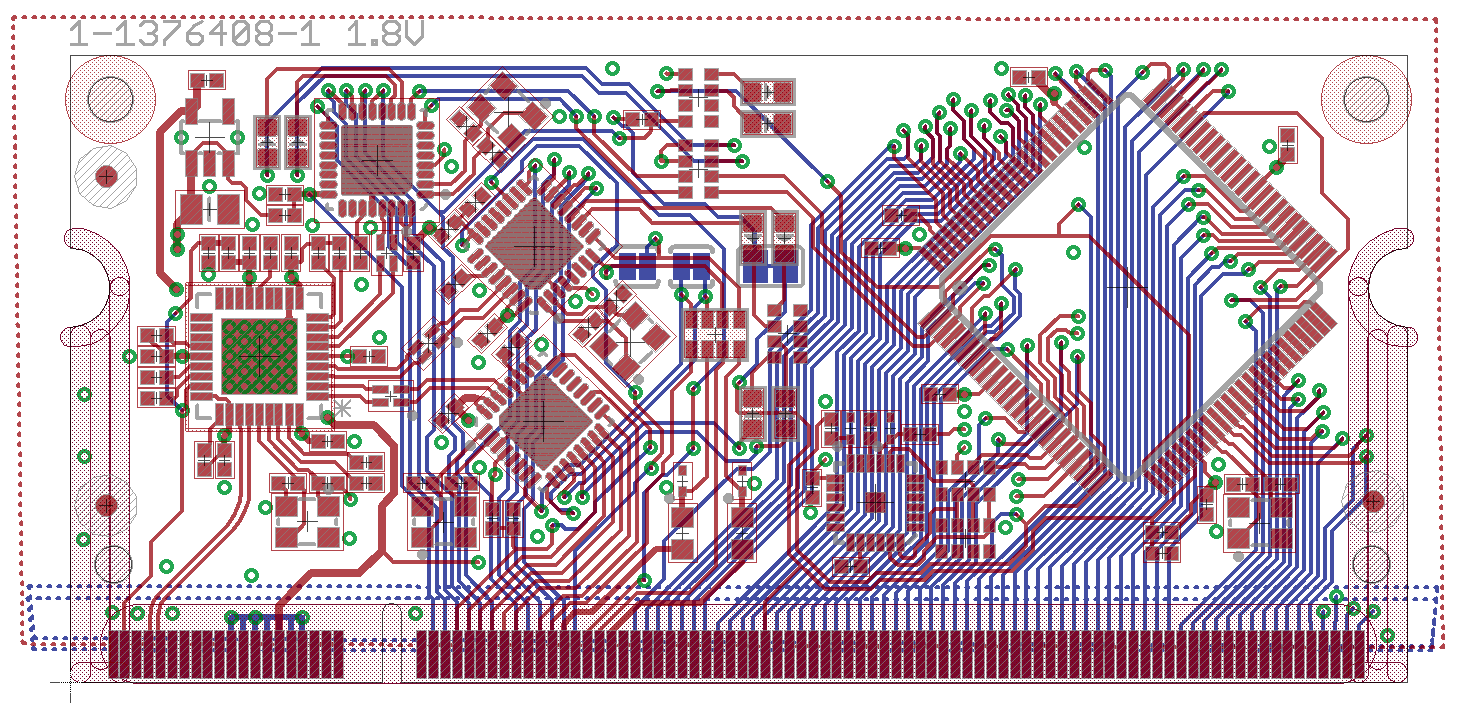
\includegraphics[height=3.5cm]{io-module.png}}
    \hfil
     \subfloat[][Size comparison between the IO board and SO-DIMM format]{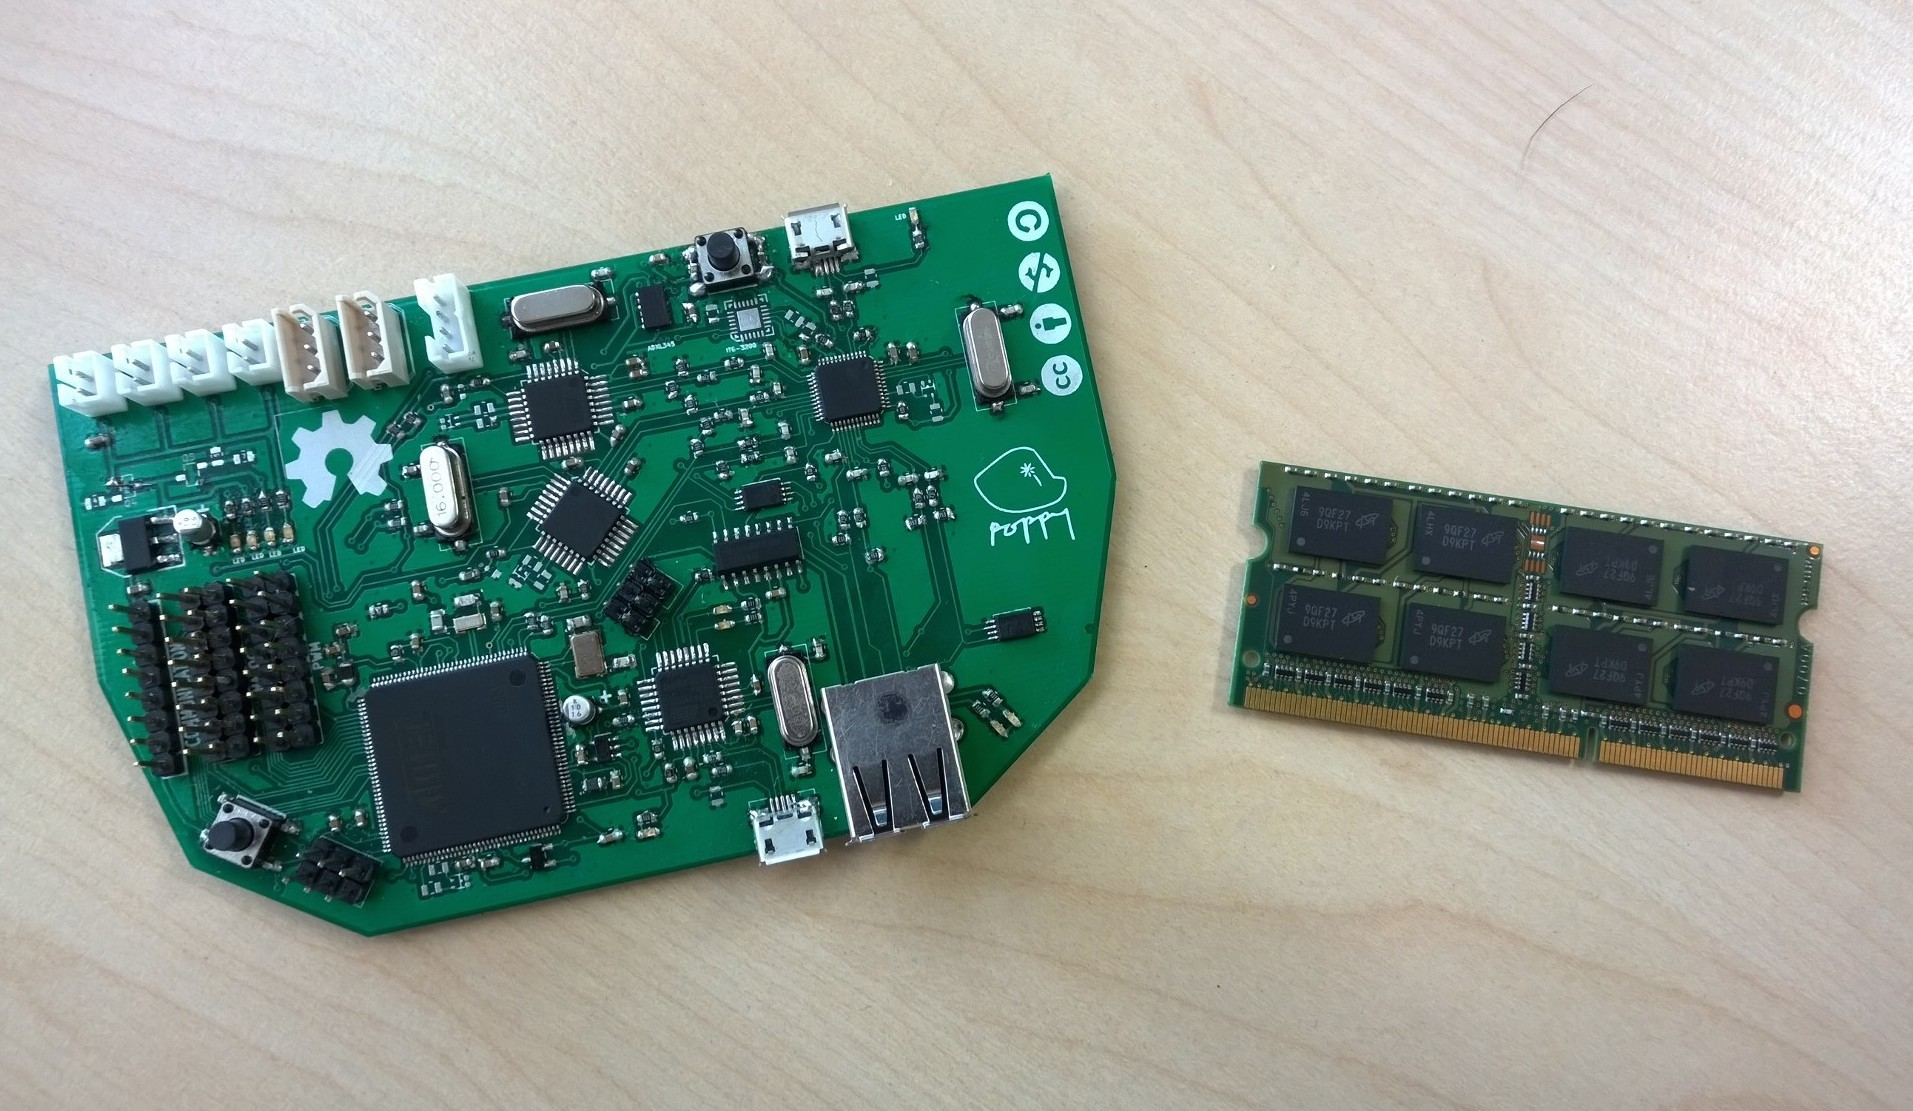
\includegraphics[height=3.5cm]{compare-io-boards.jpg}}\\
    \caption{}
    \label{fig:poppy-electronic-modularity}
\end{figure}

For the mechanics, a first step could be to split the robot into modules (e.g. head, torso, arms and legs) with defined interface. In this way, contributors could create new design while just having to ensure the interface compatibility. Therefore anyone could create a whole new head or legs system and distribute it so people can test on their Poppy.

For the electronics, we are also exploring splitting it into modules. We are working on a new design of the IO board, which will involve 2 boards, one IO module with the core of the technology we need (Arduino, motor control) and a shield with connectors.
While the shield is custom to a robot, depending on the needs and motors used, the IO module is very small and versatile so it can be integrate both in small and big robot.
The design of this IO module is already done (see REF) and is based on a DDR2 SO-DIMM format (67x30 mm) with up to 200 pins. This board involves an Arduino Mega with all its GPIO, two modified motor buses compatible for TTL and RS485 communication and an inertial unit MPU6000.



\section{Production/Distribution: an alternative approach} % (fold)

% \subsection{A research lab is not a Start-Up} % (fold)
Poppy includes three main parts: its mechatronic structure (skeleton and motors); its electronics; its software.

Reproducing and rebuilding the mechatronic structure is easy: the open-source skeleton can be printed on personal 3D printers (or using online services for higher quality printing), and motors are bought off-the-shelf (motors are currently not open-source, but very standard). Obtaining and using the software is very easy: just download on the Poppy web site.

But the fabrication of electronics is challenging. It is not yet possible to produce electronics components at home, and many institutional users do not have the competence or motivation to do so. There are some kickstarter projects going on a way to facilitate the process, yet they are not ready and won't be ready until a couple of years.

The current classical approach to build and distribute this electronics boards is to raise funding allowing the manufacturing of hundreds of boards which can then be sold by a distribution company. But a french research institute like Inria is not a distributor,  is not even legally allowed to do.

Furthermore, even if one could buy or build easily all components, some users (e.g. artists) might want to obtain and use an already fully assembled Poppy robot. Thus, a structure capable of building and distributing the electronics, as well as the mechatronics and/or the robot fully assembled is needed.

Yet, the mission of a research team at Inria is to do research, and find ways to apply and transfer the results of this research, but not directly to produce and sell a commercial product. If a commercial product can emerge from our research, one way to exploit it is to create a start-up company which will set up a business plan around it, probably based on a production in Asia and then a worldwide distribution to research laboratories, universities and fablabs (see Figure \ref{fig:classic})

\begin{figure}[ht]
    \begin{center}
        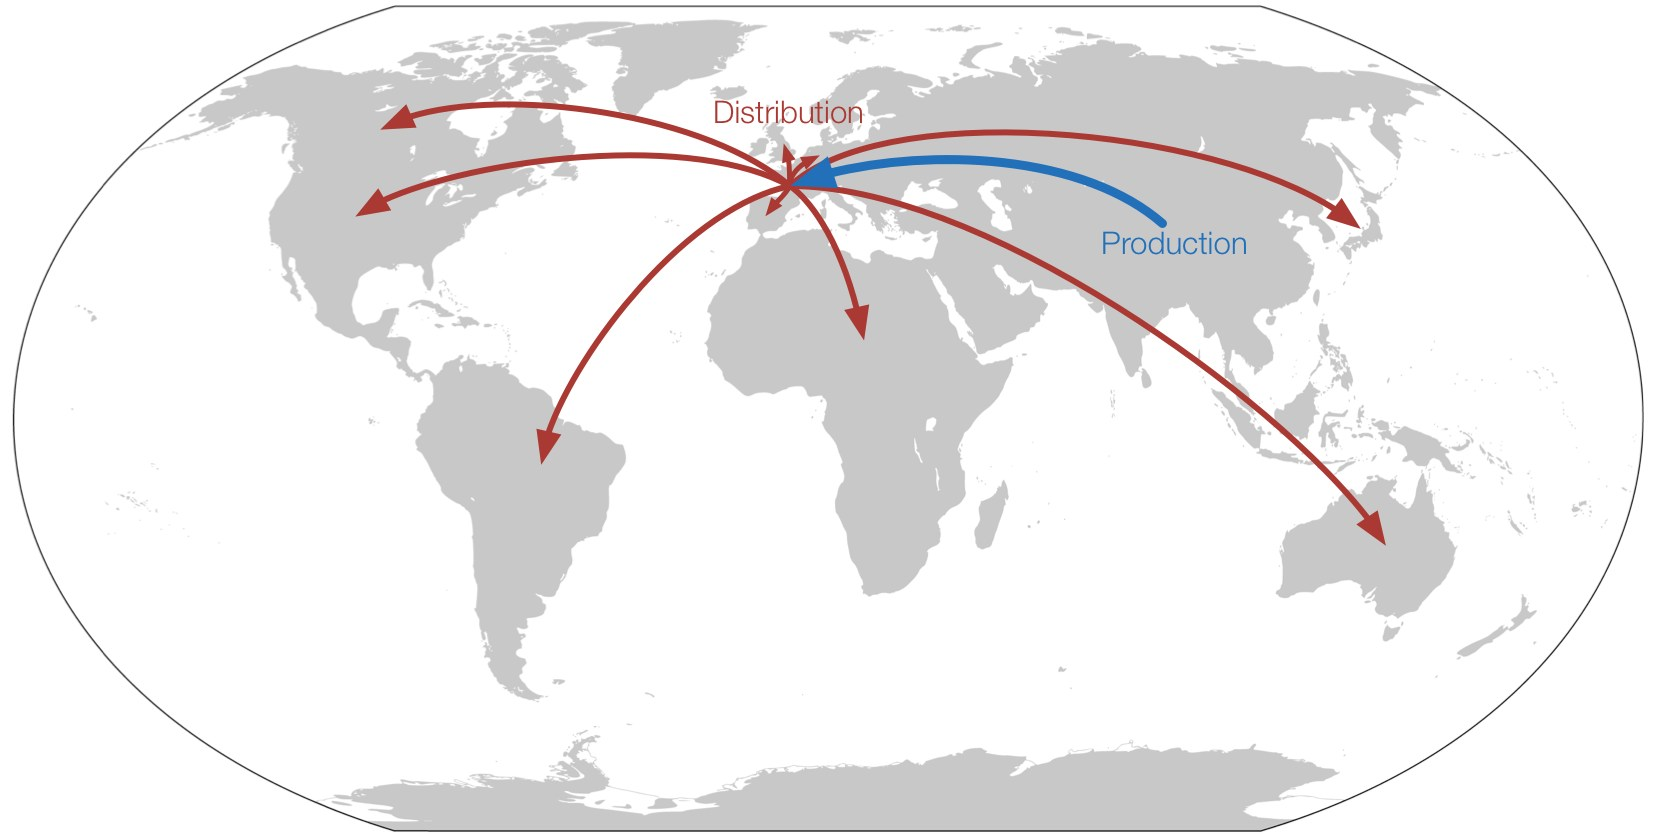
\includegraphics[width=14cm]{classic_production_distribution.jpg}
    \end{center}
    \caption{Classical approach for technology production and distribution}
    \label{fig:classic}
\end{figure}


But Poppy is not designed to be a standard commercial product. While it might foster the creation of an economical ecosystem and jobs, its main purpose is to become an educational tool that remains open, as well as rather low cost and easily reproducible. If the goal would have been to make it profitable, it would be necessary to sell it at a much higher price. The robot wouldn't be as accessible at it should to ensure the achievement of its scientific diffusion and educational missions... We would loose the intrinsic purpose of Poppy.

\subsection{Toward local open factories } % (fold)

Meanwhile, the "makers revolution" is gaining momentum~\parencite{anderson2012makers} and more and more Fablabs are created around the world. As a main mission of Poppy is to be a educational platform, Poppy could become a popular platform used, hacked, transformed within the natural FabLab activities. But also, and this is the direction explored below,  it would make sense that Poppy, as a whole or subsets of its components, be produced and distributed by Fablabs, and thus becoming a tool used by Fab Lab to develop and robustify the economic ecosystem in which they live.

\subsection{Toward an alternative model} % (fold)

An original and constructive organizational process would be to take advantage of the production phase for educational purposes. In this context, each fablab would have the possibility to produce, assemble and sell Poppy to local actors (see Figure \ref{fig:world_fab}). Thus the production phase can become a training support for the use of 3D printing techniques and the manufacturing of electronic circuits, and later on be exploited through selling the constructed platforms.


\begin{figure}[tb]
    \begin{center}
        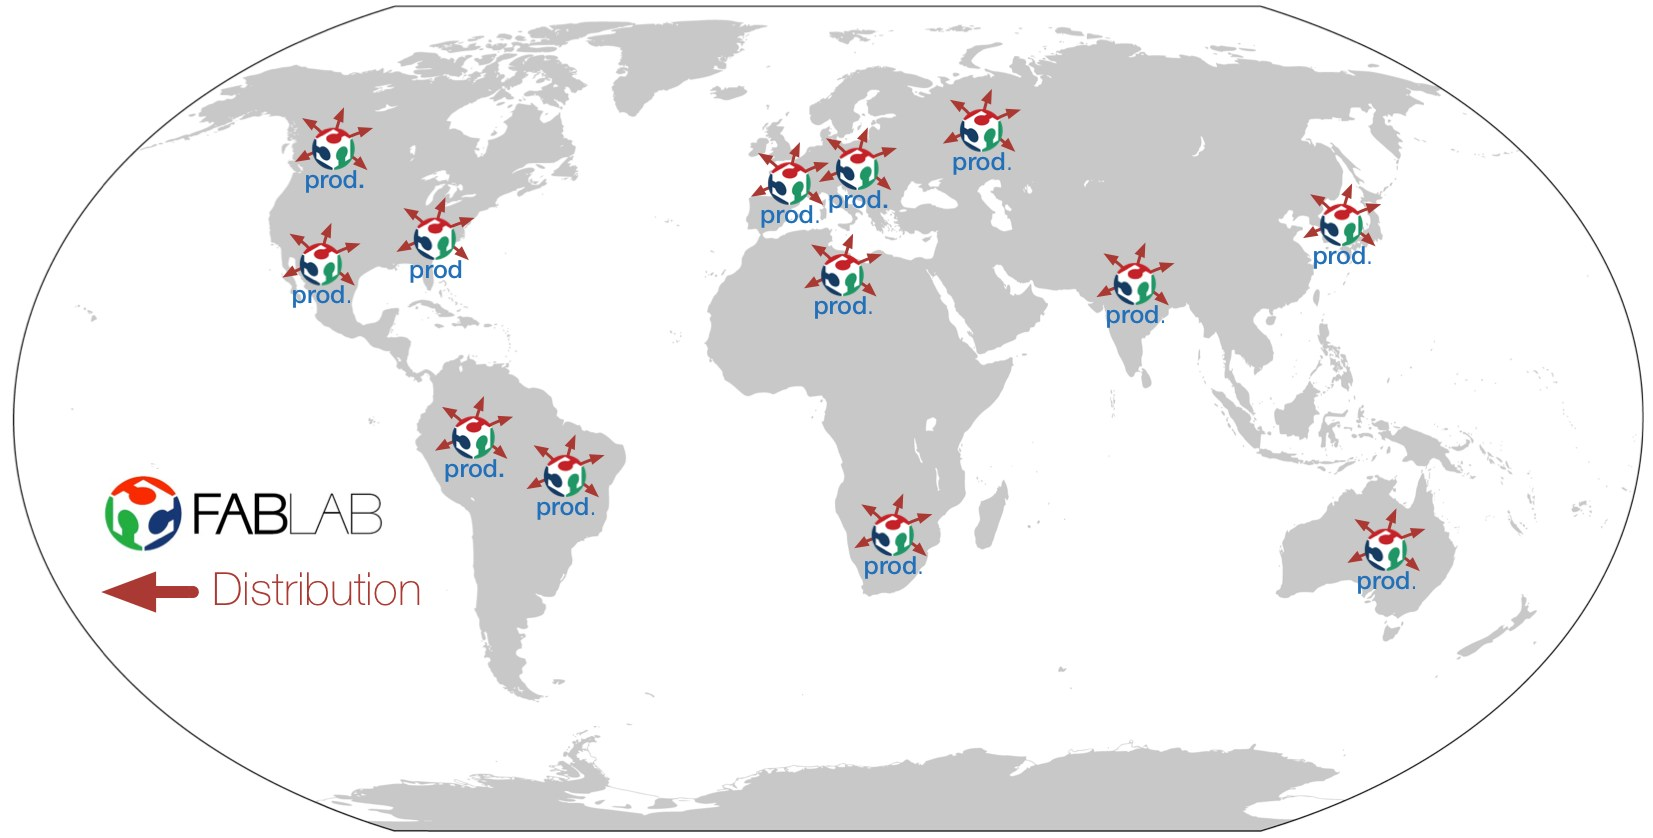
\includegraphics[width=14cm]{fabusine_distribution_world.jpg}
    \end{center}
    \caption{Fabrication and distribution locally done by Fablabs}
    \label{fig:world_fab}
\end{figure}


Also in a context where fablabs need to find an economic model, several sources of income may be found thanks to the distribution of platforms such as Poppy. The first and most obvious one is the sale to local actors of fully-assembled and functional Poppy robots produced by the Fablab. But a more advanced model can emerge. Poppy is a development robotic platform: it means that it can and will be broken, meaning that Fablabs may extend theirs commercial offers. Among them we can cite:

\begin{itemize}
    \item Ensure a support (repairs, upgrades, ...) and may sell maintenance contracts with labs/school/university and even other 3rd party FabLabs.
    \item Provide a customisation service to adapt Poppy to specific needs (e.g. a university or lycée that would like to have a Poppy on wheels rather than legs)
    \item For an event or artist residency: The FabLab could rent a robot and provide a technician,
    \item Propose profesional formation to 3D printing to companies
    \item ...
\end{itemize}

From these kinds of interaction, links and collaboration between local actors and Fablabs may emerge leading to other potentially funded projects.

\subsection{Promote local collaboration} % (fold)

Beyond the act of production and sales, Poppy could become a pretext to promote the linkage and exchange between local actors from multiple backgrounds. At the scale of a city or region, we can easily imagine a distribution of roles where several FabLabs could collaborate to build and distribute different parts of Poppy depending on their motivations, skills and equipements.
Also, it helps to connect the fablabs with local actors, public/private research labs, companies, schools/universities or artists (see Figure \ref{fig:local_synergy})

\begin{figure}[tb]
    \begin{center}
        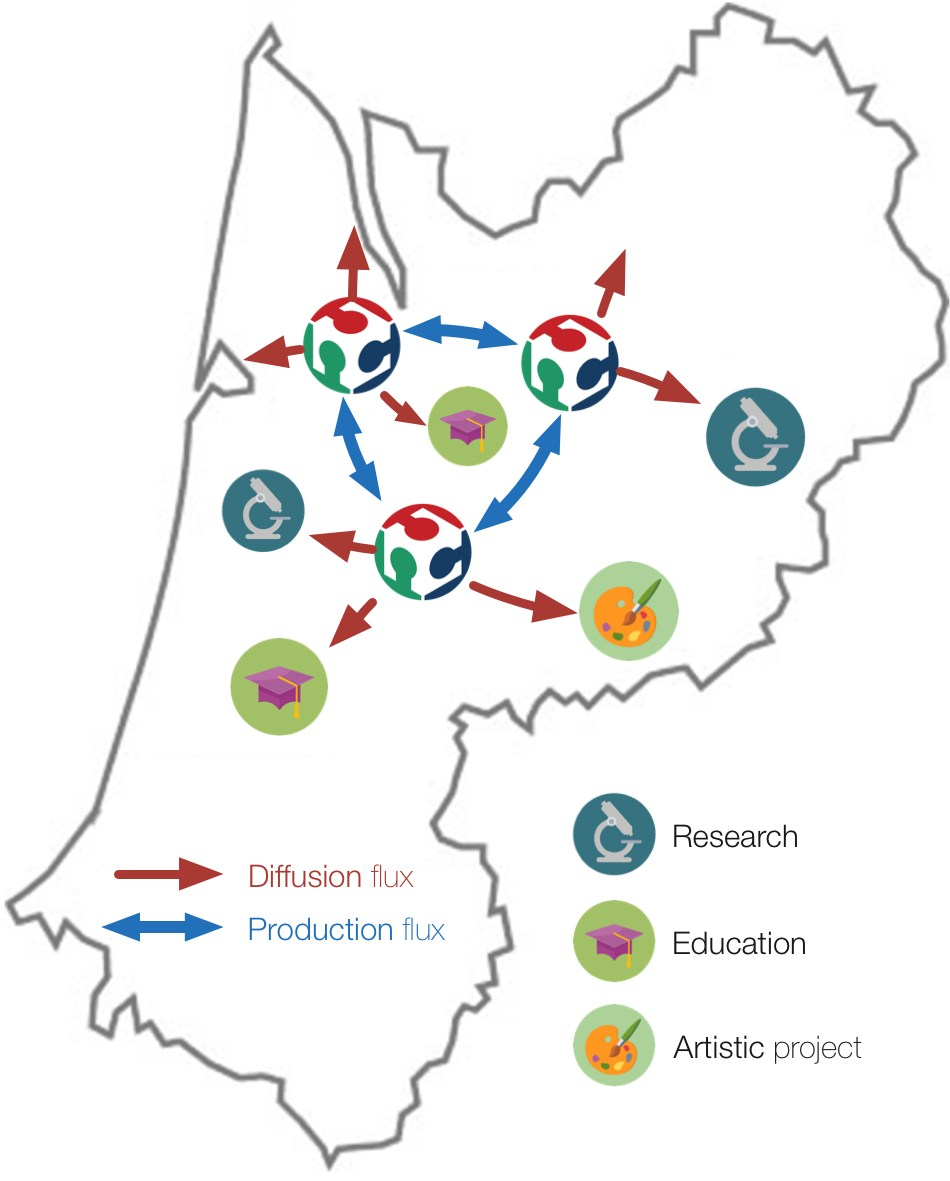
\includegraphics[height=10cm]{fabusine_local.jpg}
    \end{center}
    \caption{A synergy can emerge between Fablabs and local actors}
    \label{fig:local_synergy}
\end{figure}

\subsection{What is the role of the Flowers research team in such a process? } % (fold)

The Flowers research team's role remains essential. As the founders, designers and leaders of both the technological platform and its surrounding philosophy of openness and innovation, the Flowers team continues to improve the platform, take a central role in animating the community of users, and design new uses with scientists, educators, geeks and artists. Within this process, the Flowers team also coordinates the growing of the community of contributors and users, and designs strategies to ensure both the quality and sustainable development of the platform and its uses.

Among the tools used by the Flowers team to ensure such quality and sustainable development is through the control of the "Poppy" brand, and through policies/charters:

\begin{itemize}
\item The "Poppy" brand is owned by Inria, and the use of the brand by 3rd parties like FabLabs will only be possible through agreements ensuring that the Poppy project policies and philosophy is implemented;
\item Agreements take the form of charters/policies between Inria and FabLabs specifying guidelines to follow to ensure both quality and that each party (Inria, FabLab, users) finds its interest.
\end{itemize}

On the Inria side, the creation of an association which role would be to spin-off this technology development, community animation and quality control, is under consideration.


\subsection{conclusion} % (fold)
Poppy can be one of the first project launching this new kind of production and distribution process. The last months we met several of the main French FabLab. While their are quite enthousiast with this idea, the organisation is not completely ready to go on this way and we will certainly have to use the two ways to distribute Poppy. The first ones will be to let reseller create kit and sold them.





